\documentclass{jsarticle}

\usepackage{listings,jlisting}
\usepackage[dvipdfmx]{graphicx}
\usepackage{bmpsize}
\usepackage{bm}

\lstset{
    basicstyle={\ttfamily},
    identifierstyle={\small},
    commentstyle={\smallitshape},
    keywordstyle={\small\bfseries},
    ndkeywordstyle={\small},
    stringstyle={\small\ttfamily},
    frame={tb},
    breaklines=true,
    columns=[l]{fullflexible},
    numbers=left,
    xrightmargin=0zw,
    xleftmargin=3zw,
    numberstyle={\scriptsize},
    stepnumber=1,
    numbersep=1zw,
    lineskip=-0.5ex
}
\begin{document}

\title{計算機科学実験及演習4 エージェント 課題2}
\author{1029-28-2473 二見 颯}
\maketitle

\section{プログラム概要}
課題1で提出したハードマージンSVMに加え、ソフトマージンSVMを新しく実装した。
モデルの評価のために、K-fold交差検証を行えるようにして、
特にGaussカーネルSVMについて
予測精度が最大となる最適なハイパーパラメータの組を求めた。
データの正規化にも対応した。

\section{外部仕様}
\begin{itemize}
    \item main.py - プログラムのエントリポイント。svc.py の SoftSVM, HardSVM および utils.py を参照
    \item svc.py - SVM のクラス HardSVM と SoftSVM を実装
    \item utils.py - load\_data, plot\_decision\_regions(課題1で説明)と cross\_val\_score を実装
    \item scaler.py - MinMaxScaler(正規化)のクラスを実装
    \item extra\_data.py - iris, wine のデータセットの読み込み(sklearn.dateset)
    \item grid\_search.py - Gaussカーネルのパラメータ探索(Grid Search)を行うエントリポイント
\end{itemize}
プログラムの実行は \\
{\bf ./main.py [入力ファイルへのパス] [-h or -s] ([param c]) [-n or -p or -g] ([param kernel])} \\ 
-h or -sでハードマージンSVMを用いるかソフトマージンSVMを用いるか指定できる。また、ソフトマージンの場合、
次の[param c]にハイパーパラメータ$C$の値を指定する。
以降はカーネルトリックの種類を指定できる。(課題1と同様) \\
以下はwineのデータセットを読み込んでソフトマージンSVM(C=0.5, 多項式カーネル, p=2.0)で分類する例である。
\begin{lstlisting}
$ ./main.py WINE -s 0.5 -p 2.0
cvxopt.solvers.qp: optimization succeeded
free support vectors: 
[8, 19, 20, 24, 56, 67, 76, 86]
theta candidates:  [0.7084021246199819, 0.7084772707203442, 0.7139007303715856, 0.7084021045024342, 0.7084031399344815, 0.7084020933321371, 0.7084021065508526, 0.7084021134414269]
SoftSVM W = [ 0.08830887  0.14967919  0.30510515  0.14495329  0.05914639 -0.05083011
 -0.44413318 -0.1192389  -0.05448695  0.33204266 -0.31927956 -0.29917772
  0.10649366], θ = 0.7090989604341555
fold 1/5 accuracy:  0.9565217391304348
cvxopt.solvers.qp: optimization succeeded
free support vectors: 
[14, 55, 71, 76, 83, 86, 89]
theta candidates:  [0.5551587893610854, 0.555158796964597, 0.5551588093446753, 0.5551330327872295, 0.5551588059114891, 0.5551587847676993, 0.5551739666156776]
SoftSVM W = [ 0.21289342  0.1781607   0.17853386  0.08075174 -0.00679296 -0.09959914
 -0.4139207   0.01840754 -0.12596927  0.36167288 -0.33568391 -0.2357181
 -0.0552378 ], θ = 0.5551572836789219
fold 2/5 accuracy:  0.9565217391304348
cvxopt.solvers.qp: optimization succeeded
free support vectors: 
[21, 25, 33, 39, 55, 86]
theta candidates:  [0.2900072784299388, 0.2900072655921049, 0.2900070578429528, 0.2900072521962018, 0.290007251049357, 0.2900075710726191]
SoftSVM W = [ 0.17098488  0.14964371  0.21914376  0.05477262  0.05176998 -0.27826677
 -0.41480433 -0.0469668  -0.13237087  0.315096   -0.27987994 -0.34633944
  0.17770832], θ = 0.2900072793638624
fold 3/5 accuracy:  0.9565217391304348
cvxopt.solvers.qp: optimization succeeded
free support vectors: 
[14, 21, 25, 43, 83, 84]
theta candidates:  [0.4719949477180161, 0.4719949434207287, 0.4719949346704695, 0.47199493866718045, 0.471994950047387, 0.4719949557813248]
SoftSVM W = [ 0.18554927  0.11934352  0.2010267   0.16951661 -0.01044494 -0.05299243
 -0.38467209 -0.05042564 -0.09414849  0.3313893  -0.32498772 -0.31812269
  0.01811681], θ = 0.4719949450508511
fold 4/5 accuracy:  0.9565217391304348
cvxopt.solvers.qp: optimization succeeded
free support vectors: 
[21, 25, 33, 39, 90]
theta candidates:  [0.766548728211689, 0.7665727737412085, 0.766548733862761, 0.7665487398395889, 0.7665487288003439]
SoftSVM W = [ 0.21294178  0.12010485  0.24139871  0.13779676  0.09656673 -0.08730936
 -0.2859088  -0.09577348 -0.3040062   0.38560585 -0.3594145  -0.25748461
  0.0515577 ], θ = 0.7665535408911183
fold 5/5 accuracy:  1.0
5-fold average accuracy:  0.9652173913043478
\end{lstlisting}
\section{内部仕様}
課題1との差分について報告する
\subsection*{HardSVMクラス(svm.py)}
課題1の SVClassfier が HardSVM にあたる
\subsection*{SoftSVMクラス(svm.py)}
ソフトマージンSVMを定義する
\begin{itemize}
    \item X, y - 訓練データ点とその正解クラス
    \item n - 訓練データの個数
    \item kf - kernel trickとして用いる関数(kernel function)
    \item p - kernel functionのパラメータ(optional)
    \item C - ソフトマージンSVMで誤識別に対するペナルティの強さを表すパラメータ
    \item alpha, theta - SVMの内部パラメータであり、それぞれsetLagrange関数, setClassifier関数で決定する
\end{itemize}
コンストラクタにより、kf, p, Cを決定する
\subsection*{fit}
X, y, nを決定して、alpha, thetaを決定する各関数を呼び出す \\
@param[in] X, y

\subsection{\_setLagrange}
ソフトマージン利用の場合の最適化問題は、
\begin{eqnarray}
\max \{\sum_{k=0} \alpha_k - \sum_{k=0} \sum_{l=0} \alpha_k y_k \alpha_l y_l K(\bm{x_k}, \bm{x_l}) / 2\} \\
(\sum_{k=0} \alpha_k y_k = 0, 0 < \alpha_k < C)
\end{eqnarray}
となる。cvxopt.solvers.qp において、例えば $\alpha$ が2次元のときに以下のようにG, hを定めた。
\begin{eqnarray}
    \left(
        \begin{array}{ccc}
          -1 & 0 \\
          0 & -1 \\
          1 & 0 \\
          0 & 1 
        \end{array}
      \right)
    \left(
        \begin{array}{ccc}
          \alpha_1 \\
          \alpha_2
        \end{array}
      \right)
    =
    \left(
        \begin{array}{ccc}
          0 \\
          0 \\
          C \\
          C
        \end{array}
      \right)
\end{eqnarray}
\subsection{\_setClassifier}
ハードマージンSVMではサポートベクトルを 0 $<$ alpha としたが、ソフトマージンSVMでは 0 $<$ alpha $<$ C となる
自由サポートベクトルと考える。
この自由サポートベクトル点$\bm{x_i}$に関して、$\theta_i = \sum_{k=0} \alpha_k y_k K(\bm{x_k}, \bm{x_i}) - y_i$を求める。
これらがiによらず一定であることを確認して、その平均を theta とする。

\subsection*{\_kernelPolynomial, \_kernelGauss}
課題1と同様

\subsection*{predict}
SVMによりtXのクラスの予測をする \\
@param[in] tX(batch\_size * dim) テストデータ \\
SVMの識別関数は、$f(\bm{x}) = sign(\sum_{k=0} \alpha_k y_k K(\bm{x_k}, \bm{x}) - \theta)$とする。
各tX[i]について、前計算したay = $\sum_{k=0} \alpha_k y_k$ と K($\bm{x}$, tX[i]) の行列積によりこの値を計算する。

\subsection*{cross\_val\_score(utils.py)}
K-Foldの交差検証を行う \\
@param[in] X, y, model \\
@param[in] k: 分割数(k-Fold)

各分割ごとのデータのクラスラベル等の偏りを無くすため、交差検証の前にX, yをシャッフルする。
シャッフル後のX, yについて、sizeをyの要素数として、
[0, size/k), [size/k, 2 * size/k), ...とインデックスをk組に分割して、k-1組をtrain data, 1組を
test dataとすることをk回繰り返している。
また、モデルを評価する前処理として、train dataに対してMinMaxScalerを用いて正規化している。test data は
train dataと同じパラメータでスケール調整する。

\subsection*{MinMaxScalerクラス(scaler.py)}
データの正規化を行う \\
fit で与えられたデータの最小値、最大値をそれぞれmin, maxに代入して、
transform で X = (X - min) / (max - min) と変換したXを返す。

\section{評価結果}
\subsection{ソフトマージンSVMの表現力}
図1のようなデータ点集合(data/sample\_soft.dat)の場合、ハードマージンの線形SVMでは
誤識別を許容しないため、最適化問題を解くことができずSVMを構成できない。
ここで、$C$を導入して誤識別を最小化するようなソフトマージンSVMを構成すると、
このようなクラスの重なりを含むデータ点集合に対してもある程度の線形分離ができるようになる。
図1は$C = 0.5$の場合である。
\begin{figure}[!h]
\centering 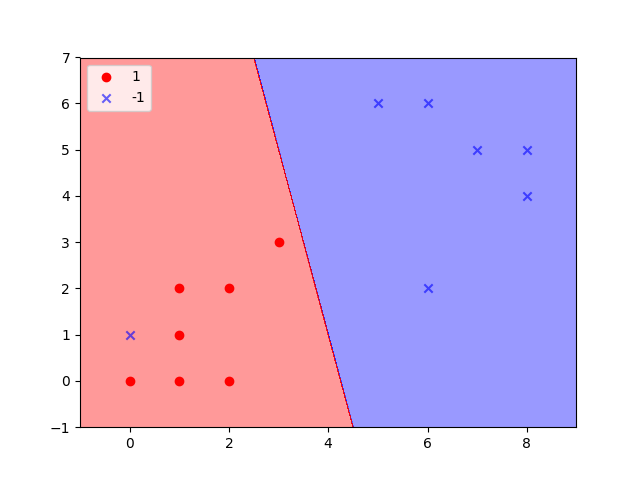
\includegraphics[width=15cm]{soft_margin.png}
\caption{soft margin example}
\end{figure}

\subsection{ハイパーパラメータ探索(Grid Search)}
sample\_circle.dat で Gauss カーネルSVMを評価することを考える。
パラメータ$p$および$C$の組の値を変更して交差検証を行い accuracy を求めた。
$p$の候補は$(2^(-7), 2^(-6), ..., 2^5)$, $C$の候補は$(2^(-3), 2^(-2), ..., 2^3)$として、13*7通りのGrid Searchを
行った。\\
図2に結果を示す。
\begin{figure}[!h]
\centering 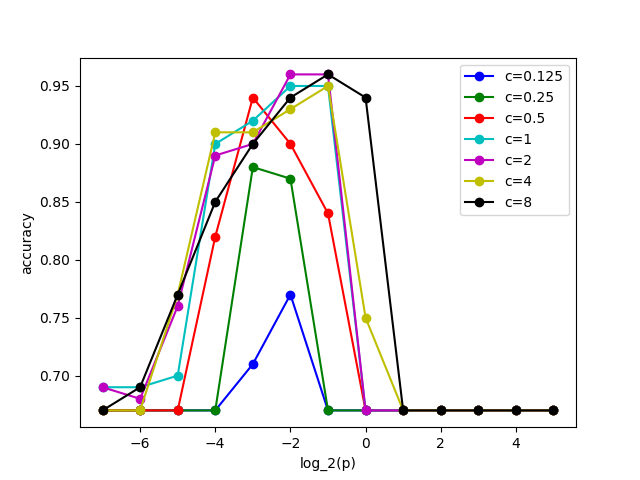
\includegraphics[width=15cm]{grid_search.png}
\caption{Grid Search}
\end{figure}
この場合最適なパラメータは、$p=0.25, C=2.0$のときで accuracy=0.96 であった。

\section{考察}
ソフトマージンSVMでは、線形識別可能でない場合に対応するためスラック変数$\xi_i$を導入する。
マージン内で正しく分類できる場合$\xi_i = 0$, マージン境界を越えるが正しく識別できる場合$0 < \xi_i <= 1$, 
識別境界を越えて誤識別される場合$\xi_i > 1$とする。
ソフトマージンSVMでは、マージンを$2 / \|\bm{w}\|$とすると、評価関数
\begin{eqnarray}
L = \bm{w}^{\mathrm{T}}\bm{w} / 2 + C \sum_{i=0} \xi_i
\end{eqnarray}
を最小化する。
パラメータCを大きくすると、$\|\bm{w}\|$の最小化、すなわちマージン最大化よりも誤識別数を最小化する方を優先するように働く。
これによって、モデルは訓練データに対して過学習しやすくなる。
パラメータCを小さくすると、逆にマージン最大化は優先されるが、誤識別は多くなり、訓練データに対して過小適合しやすくなる。
パラメータCはマージン最大化と誤識別数の最小化のトレードオフを表すパラメータといえる。

Gaussカーネルのパラメータ$\sigma(= p)$を小さくすると、モデルは訓練データに対して過学習して、
$\sigma(= p)$を大きくするとモデルは訓練データに過小適合する傾向が見られる。
例として図3は、ソフトマージンSVM(C=2.0)で$\sigma=0.02$とした場合であり、過学習していることがわかる。
\begin{figure}[!h]
\centering 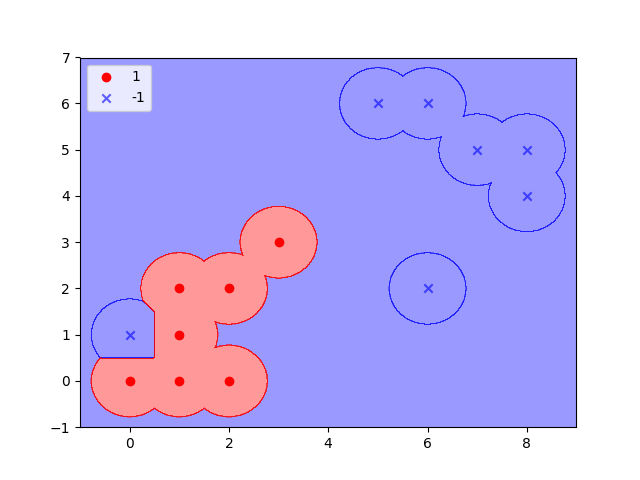
\includegraphics[width=15cm]{overfitting.png}
\caption{overfitting}
\end{figure}
SVMの識別関数は
$f(\bm{x}) = sign(\sum_{k=0} \alpha_k y_k \exp(-\|\bm{x_k}-\bm{x}\| / 2p^2) - \theta)$となる。
$\sigma$が小さい場合は入力データ$\bm{x_k}$から遠く離れているサポートベクトルが識別に寄与することになるが、
$\sigma$が大きい場合は入力データ$\bm{x_k}$近傍のサポートベクトルのみが識別に寄与することになる。これにより、
過小適合、過学習が説明できる。

最後に、sklearn.dataset.wineデータセットについて、正規化(MinMaxScaler)なし、正規化ありの場合をGrid Searchで比較した。
図4, 5に示す通り、正規化が識別性能に大きな影響を与えることがわかる。
wineデータセットでは特徴量が13あり、それぞれの値の取りうる範囲を0-1に統一することで特徴量ごとの値の取りうる範囲の違いに影響を
受けなくなるため、性能が向上すると考えられる。
\begin{figure}[!h]
\centering 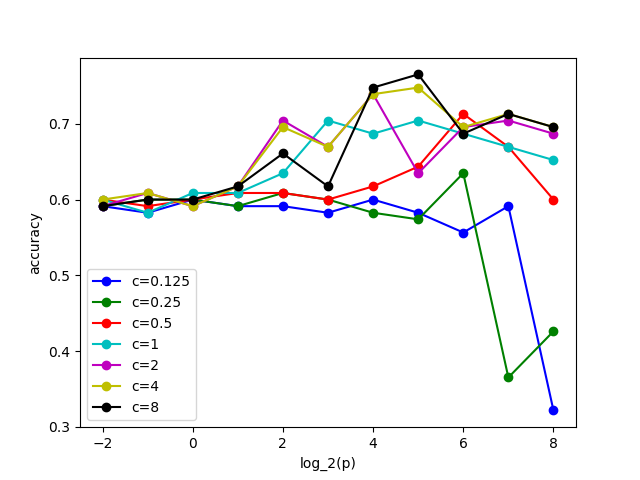
\includegraphics[width=10cm]{nostd.png}
\caption{正規化なし}
\end{figure}
\begin{figure}[!h]
\centering 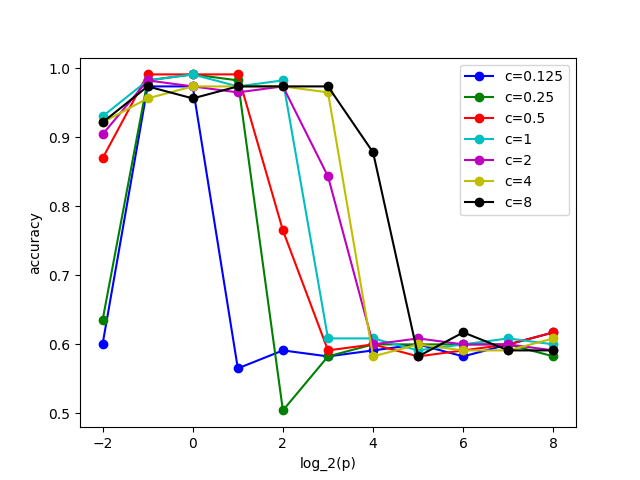
\includegraphics[width=10cm]{std.png}
\caption{正規化あり}
\end{figure}


\section{参考資料}
\begin{itemize}
    \item Python機械学習プログラミング Sebastian Raschka 著
    \item はじめてのパターン認識 平井 有三 著
    \item scikit-learnとTensorflowによる実践機械学習 Aurelien Geron 著
\end{itemize}
\end{document}